\begin{abstract}
\section*{Vorwort}
\label{sec:preface}
	Der vorliegende Text ist eine Mitschrift zur Vorlesung $\CAT$ kubische Komplexe, gelesen von Dr. Olga Varghese an der WWU Münster im Wintersemester 2015/2016. Der Inhalt entspricht weitestgehend dem Tafelanschrieb und den Vorlesungsnotizen, welche auf der Vorlesungswebsite bereitsgestellt werden. Dieses Werk ist daher keine Eigenleistung des Autors und wird nicht von der Dozentin der Veranstaltung korrekturgelesen. Für die Korrektheit des Inhalts wird keinerlei Garantie übernommen. Bemerkungen, Korrekturen und Ergänzungen kann man folgenderweise loswerden:
	\begin{itemize}
		\item persönlich durch Überreichen von Notizen oder per E-Mail
		\item durch Abändern der entsprechenden TeX-Dateien und Versand per E-Mail an mich
		\item direktes Mitarbeiten via GitHub. Dieses Skript befindet sich im \texttt{latex-wwu}-Repository von Jannes Bantje:
		\begin{center}
			\url{https://github.com/JaMeZ-B/latex-wwu}
		\end{center}
	\end{itemize}
	
	\subsection*{Literatur}
	\label{sub:lit}
	\begin{itemize}
		\item \textsc{Bridson, Haefliger}: Metric Spaces of Non-Positive Curvature \cite{BridsonHaefliger}
		\item \textsc{Serre}: Trees \cite{Serre}
		\item \textsc{Bekka, de la Harpe, Valette}: Kazhdan's Property $\prT$ \cite{BekkaHarpeValette}
	\end{itemize}
	
	\subsection*{Kommentar der Dozentin}
	In der geometrischen Gruppentheorie werden Gruppen als Symmetrien von Räumen betrachtet. Ihre algebraische Eigenschaften werden mittels geometrischer Eigenschaften der Räume, auf denen sie wirken, untersucht. Gruppen, die auf kubischen Komplexen wirken -- das sind polyhedrische Komplexe, die aus Würfeln gebaut sind -- sind dabei besonders gut verstanden.
	
	Die Vorlesung wird eine Einführung in die Strukturtheorie $\CAT$ kubischer Komplexe liefern, sowie Anwendungen in der Gruppentheorie diskutieren.
	\newpage
	
\begin{center}
		\begin{minipage}{0.3\textwidth}
		\begin{flushleft}
			\textbf{abstrakte Gruppen}
			\begin{itemize}
				\item endliche Gruppen
				\item $\GL_n(\ZZ)$, $\SL_n(\ZZ)$
				\item $\Aut(F_n)$, $\SAut(F_n)$
				\item Coxetergruppen
			\end{itemize}
		\end{flushleft}
	\end{minipage}
	~
	\begin{minipage}{0.25\textwidth}
		\begin{center}
			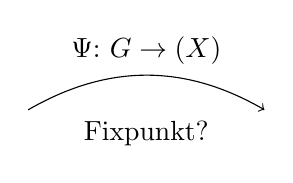
\begin{tikzpicture}
				\draw[->] (0,0) to [bend left] (3,0);
				\draw (1.5,.75) node{$\Psi \mbox{:} \ G \rightarrow \Isom(X)$};
				\draw (1.5,-.3) node{Fixpunkt?};
			\end{tikzpicture}
		\end{center}
	\end{minipage}
	~
	\begin{minipage}{0.35\textwidth}
		\begin{flushleft}
			\textbf{metrische Räume mit\\ "viel Geometrie"}
			\begin{itemize}
				\item $(\RR^n,d_2)$
				\item Hilberträume
				\item simpliziale Bäume
				\item $\CAT$ kubische Komplexe
			\end{itemize}
		\end{flushleft}
	\end{minipage}
\end{center}
	
	\subsection*{Geplante Themen}
	\begin{itemize}
		\item $\CAT$-Räume (simpliziale Bäume, kubische Komplexe)
		\item Gruppenwirkungen auf $\CAT$ kubische Komplexe
		\item \textsc{Bruhat-Tits}-Fixpunktsatz für $\CAT$ kubische Komplexe
		\item \textsc{Helly}'s Theorem
		\item Kazhdan-Eigenschaft $\prT$
	\end{itemize}
	
	\subsection*{Vorlesungswebsite}
	\label{sub:link}
	Das handgeschriebene Skript sowie weiteres Material findet man unter folgendem Link:
	\begin{center}
		\url{http://wwwmath.uni-muenster.de/u/ag_kramer/index.php?name=KubischeKomplexe_15&menu=teach&lang=de}
	\end{center}
	
	\vfill
	\begin{flushright}
		Phil Steinhorst \\
		p.st@wwu.de
	\end{flushright}
\end{abstract}